

\section{The Large Hadron Collider}

The Large Hadron Collider (LHC) is a proton-proton collider at the European OrganizItion for Nuclear Research (CERN)1, residing in the $26.7$ km tunnel originally build for the Large Electron Positron Collider (LEP).It consists of two rings with counter-rotating beams, being crossed at four interaction points, point 1, 2, 5, and 82. The proton beams are ramped up to the energy of 450 GeV by a chain of pre-accelerators, and are then injected into the LHC ring (Figure \ref{fig:CERN_complex}). The LHC is using superconducting magnets, which are, due to very restrictive space in the tunnel, dedicated to both rings at one time. One of the also superconducting cables between these magnets caused an incident in 2008, where a bad thermal connection lead to up-heating of material and liquid helium \ref{incident}. The LHC was restarted in March 2010 not running at the originally planned center-of-mass energy of 14 TeV, but at 7 TeV. With a design luminosity of L is $1034 cm^{-2}s^{-1}$, with a bunch crossing every $25 ns$. Figure \ref{fig:LHC_xsec} shows the total cross section prospects for LHC in comparison with several Standard Model processes. In 2012 LCH delivered a total luminosity of 23.30 $fb^{-1}$ as shown on \ref{fig:lumi_2012}.

Several experiments are hosted at the LHC. ATLAS (A Toroidal Lhc ApparatuS) \ref{atlas} and CMS (Compact Muon Solenoid) \ref{cms} are multi-purpose detectors, aiming at Stan- dard Model physics including higgs searches and physics beyond the Standard Model. LHCb \ref{lhcb} is dedicated to b-quark physics and the related problem of CP violation the matter-antimatter asymmetry in the universe. As the LHC can also be run in heavy ion (lead-lead) collision mode, one experiment, ALICE (A Large Ion Collider Experiment) \ref{alice}, focuses on strongly interacting matter and quark-gluon plasma. Finally, another two experiments, LHCf \ref{lhcf} and TOTEM (TOTal Elastic and diffractive cross section Measurement) \ref{totem} are designed to study the total proton-proton interaction cross-section. The site for each of the previously mentioned experiments is shown in Figure \ref{fig:CERN_complex}.

The high luminosity and bunch crossing rate allows 


\begin{figure}[tbh!]
	\centering
	\begin{tabular}{cc}
		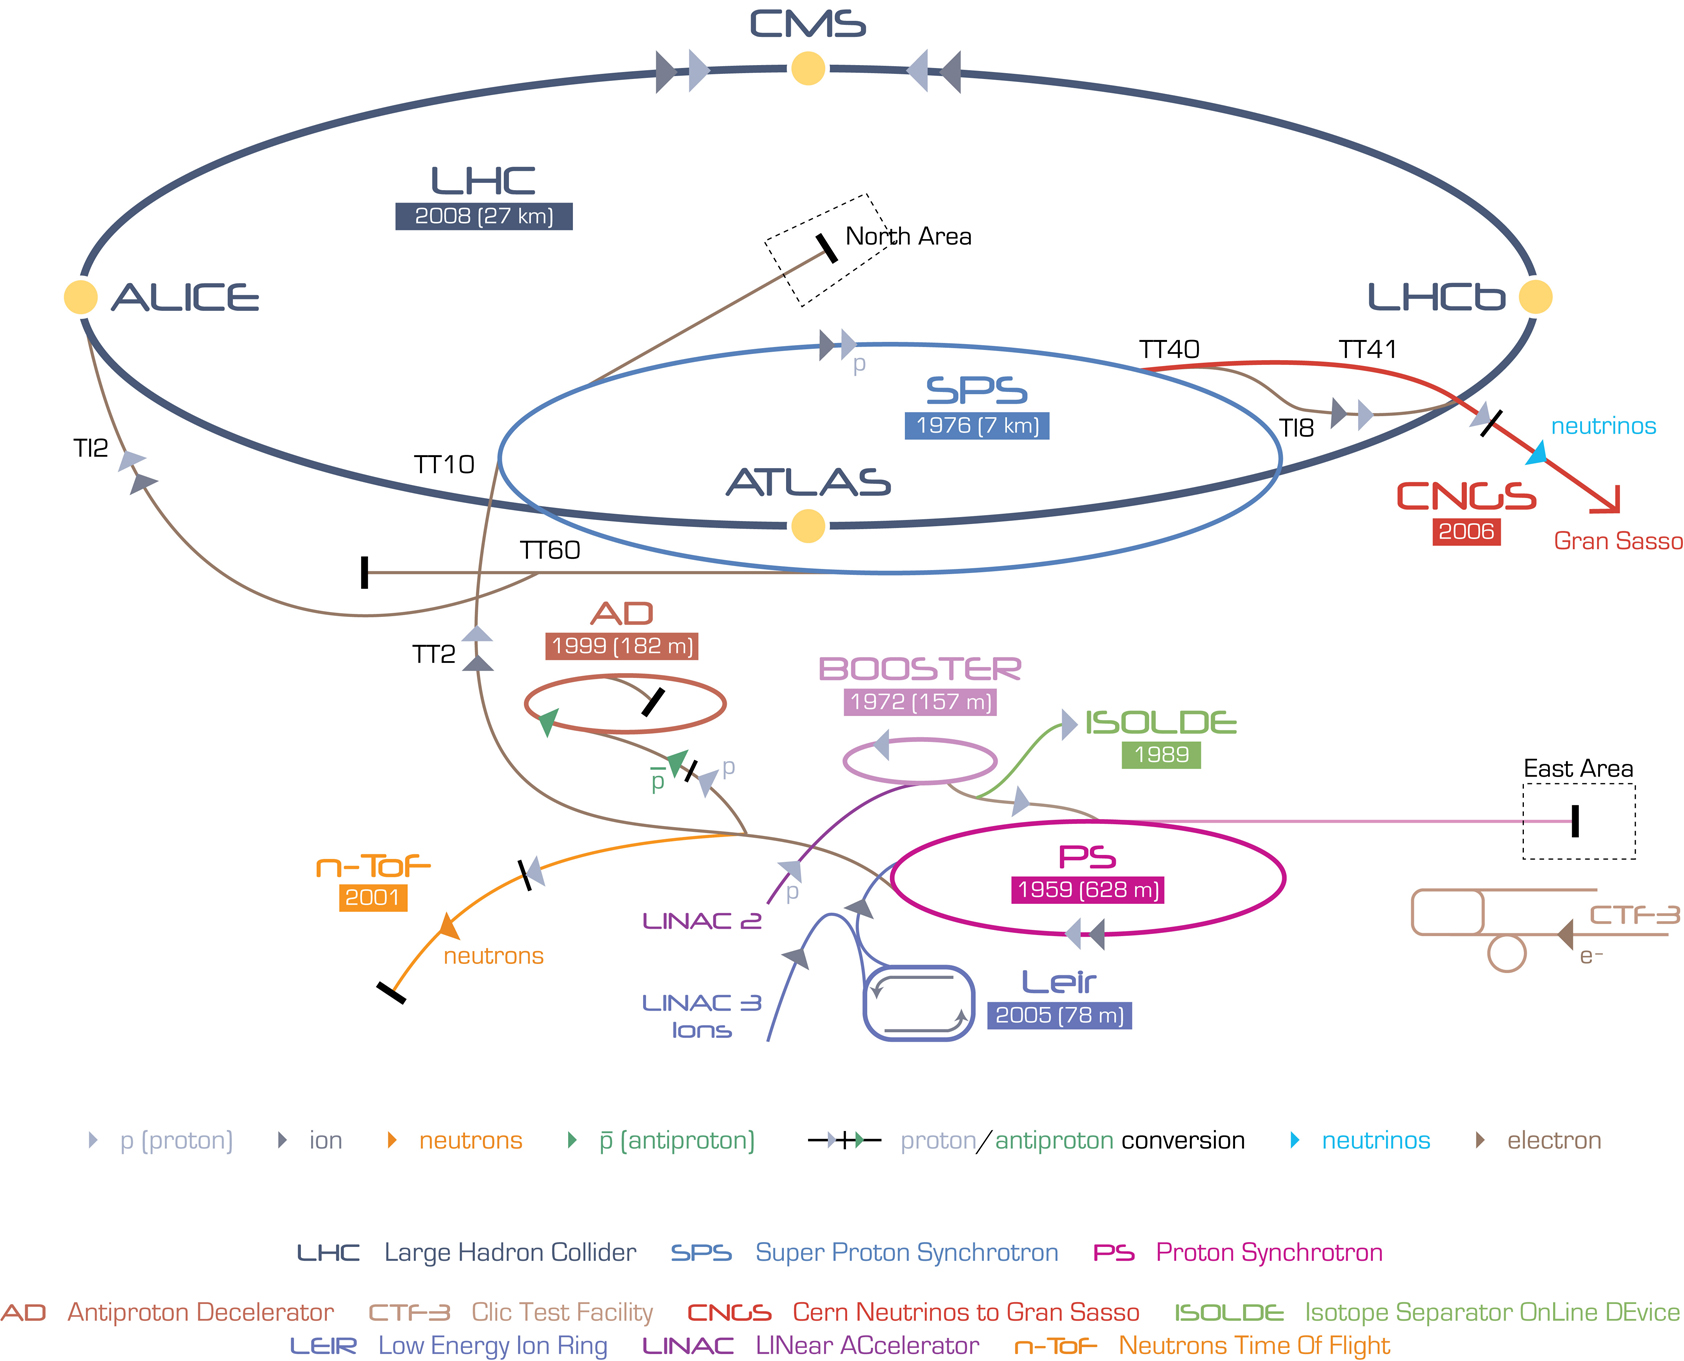
\includegraphics[width=0.75\textwidth]{detector/pics/CERN_complex.jpg}
	\end{tabular}
	\caption{Schematic view of the LHC with its four big experiments. Also shown are the pre-accelerators, as well as several other experiments operated at CERN.}
	\label{fig:CERN_complex}
\end{figure}

\begin{figure}[tbh!]
	\centering
	\begin{tabular}{cc}
		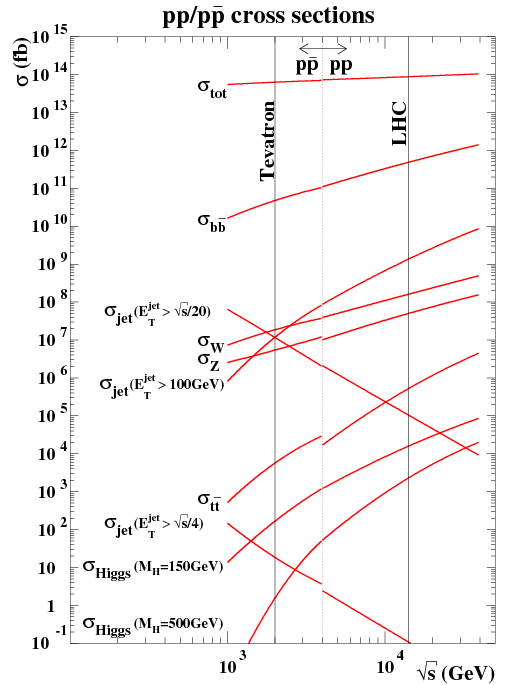
\includegraphics[width=0.75\textwidth]{detector/pics/LHC_xsec.png}
	\end{tabular}
	\caption{Production cross-sections for several representative processes at hadron colliders as a function of the machine center-of-mass energy}
	\label{fig:LHC_xsec}
\end{figure}

\begin{figure}[tbh!]
	\centering
	\begin{tabular}{cc}
		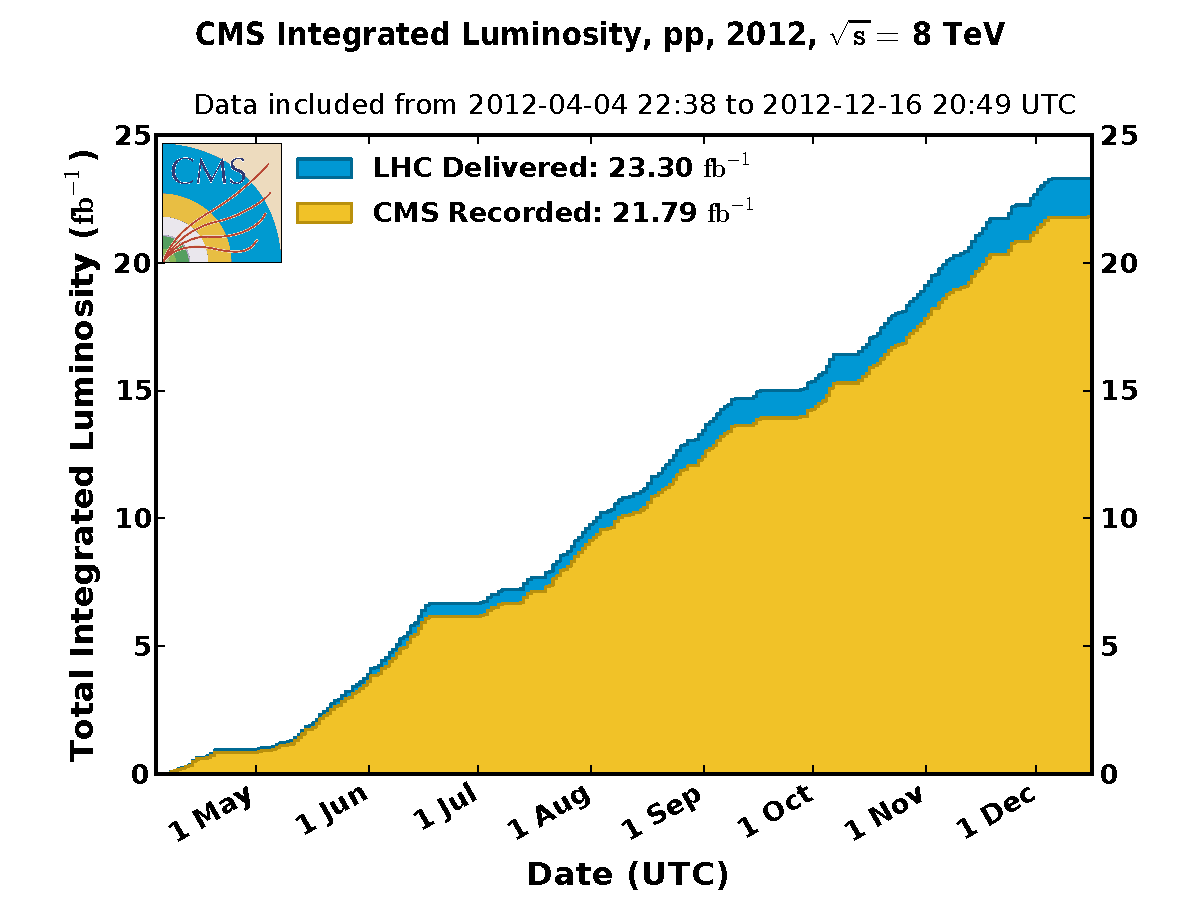
\includegraphics[width=0.75\textwidth]{detector/pics/int_lumi_per_day_cumulative_pp_2012.pdf}
	\end{tabular}
	\caption{Cumulative luminosity versus day delivered to (blue), and recorded by CMS (orange) during stable beams and for p-p collisions at 8 TeV centre-of-mass energy in 2012. The delivered luminosity accounts for the luminosity delivered from the start of stable beams until the LHC requests CMS to turn off the sensitive detectors to allow a beam dump or beam studies. Given is the luminosity as determined from counting rates measured by the luminosity detectors. These detectors have been calibrated with the use of the van-der-Meer beam-separation method, where the two beams are scanned against each other in the horizontal and vertical planes to measure their overlap function.}
	\label{fig:lumi_2012}
\end{figure}

\section{The CMS Experiment}

The Compact Muon Solenoid is a "general purpose" experiment placed at Point 5 along the LHC ring. The experiment has a cylindrical geometry and is divided in two main sections: the lateral section, called Barrel and the remaining ones called Endcaps (Figure \ref{fig:CMS_apparatus}).   
CMS was designed to fulfill the following important research tasks:
\begin{enumerate}
	\item Search for the Higgs Boson
	\item Search for physics beyond the standard model
\end{enumerate}
those tasks combined with the LHC design specifications require a detector with the following characteristics:
\begin{itemize}
	\item High granularity and response;
	\item High radiation damage resistance;
	\item Good performances in the reconstruction of the $\mu$ particle charge, momentum and invariant mass;
	\item Good $\tau$ particle and jets reconstruction efficiency;
	\item High resolution on the combined reconstruction of electrons and photons;
	\item Great phase-space coverage $|\eta| < 5$;
	\item Good resolution in the missing transverse energy reconstruction.
\end{itemize} 

The CMS detector has a $24 m$ length and a $14.6 m$ diameter for a total wight of $14500 t$. The experiment is made of several sub-detectors placed concentrically around the interaction point, each one providing complementary measurements (Figure \ref{fig:CMS_slice}). Particles coming from the interaction point first go through the tracking system witch measures the position of charged particles hitting its layers. The calorimeters are places right outside the tracking system and are capable of measuring the particles energy deposits. The Electromagnetic Calorimeter (ECAL) measure the energy of electrons and photons, the Hadronic Calorimeter (HCAL) measures the energy of all fermions containing quarks.

The most important section in the detector is the high magnetic field which allows the measurement of high momentum charged particles with high precision. Measurements with high resolution standards requires high magnetic fields, therefore the choice to use superconducting technology for the magnets. All previously introduced sub-detectors are contained inside the solenoid superconducting magnet. All particles except for $\mu$ and low interacting ones get contained by the calorimeters and the magnetic return yoke. Outside the magnet there are the muon chambers witch identify $\mu$ particles and measure their momentum.

\begin{figure}[tbh!]
	\centering
	\begin{tabular}{cc}
		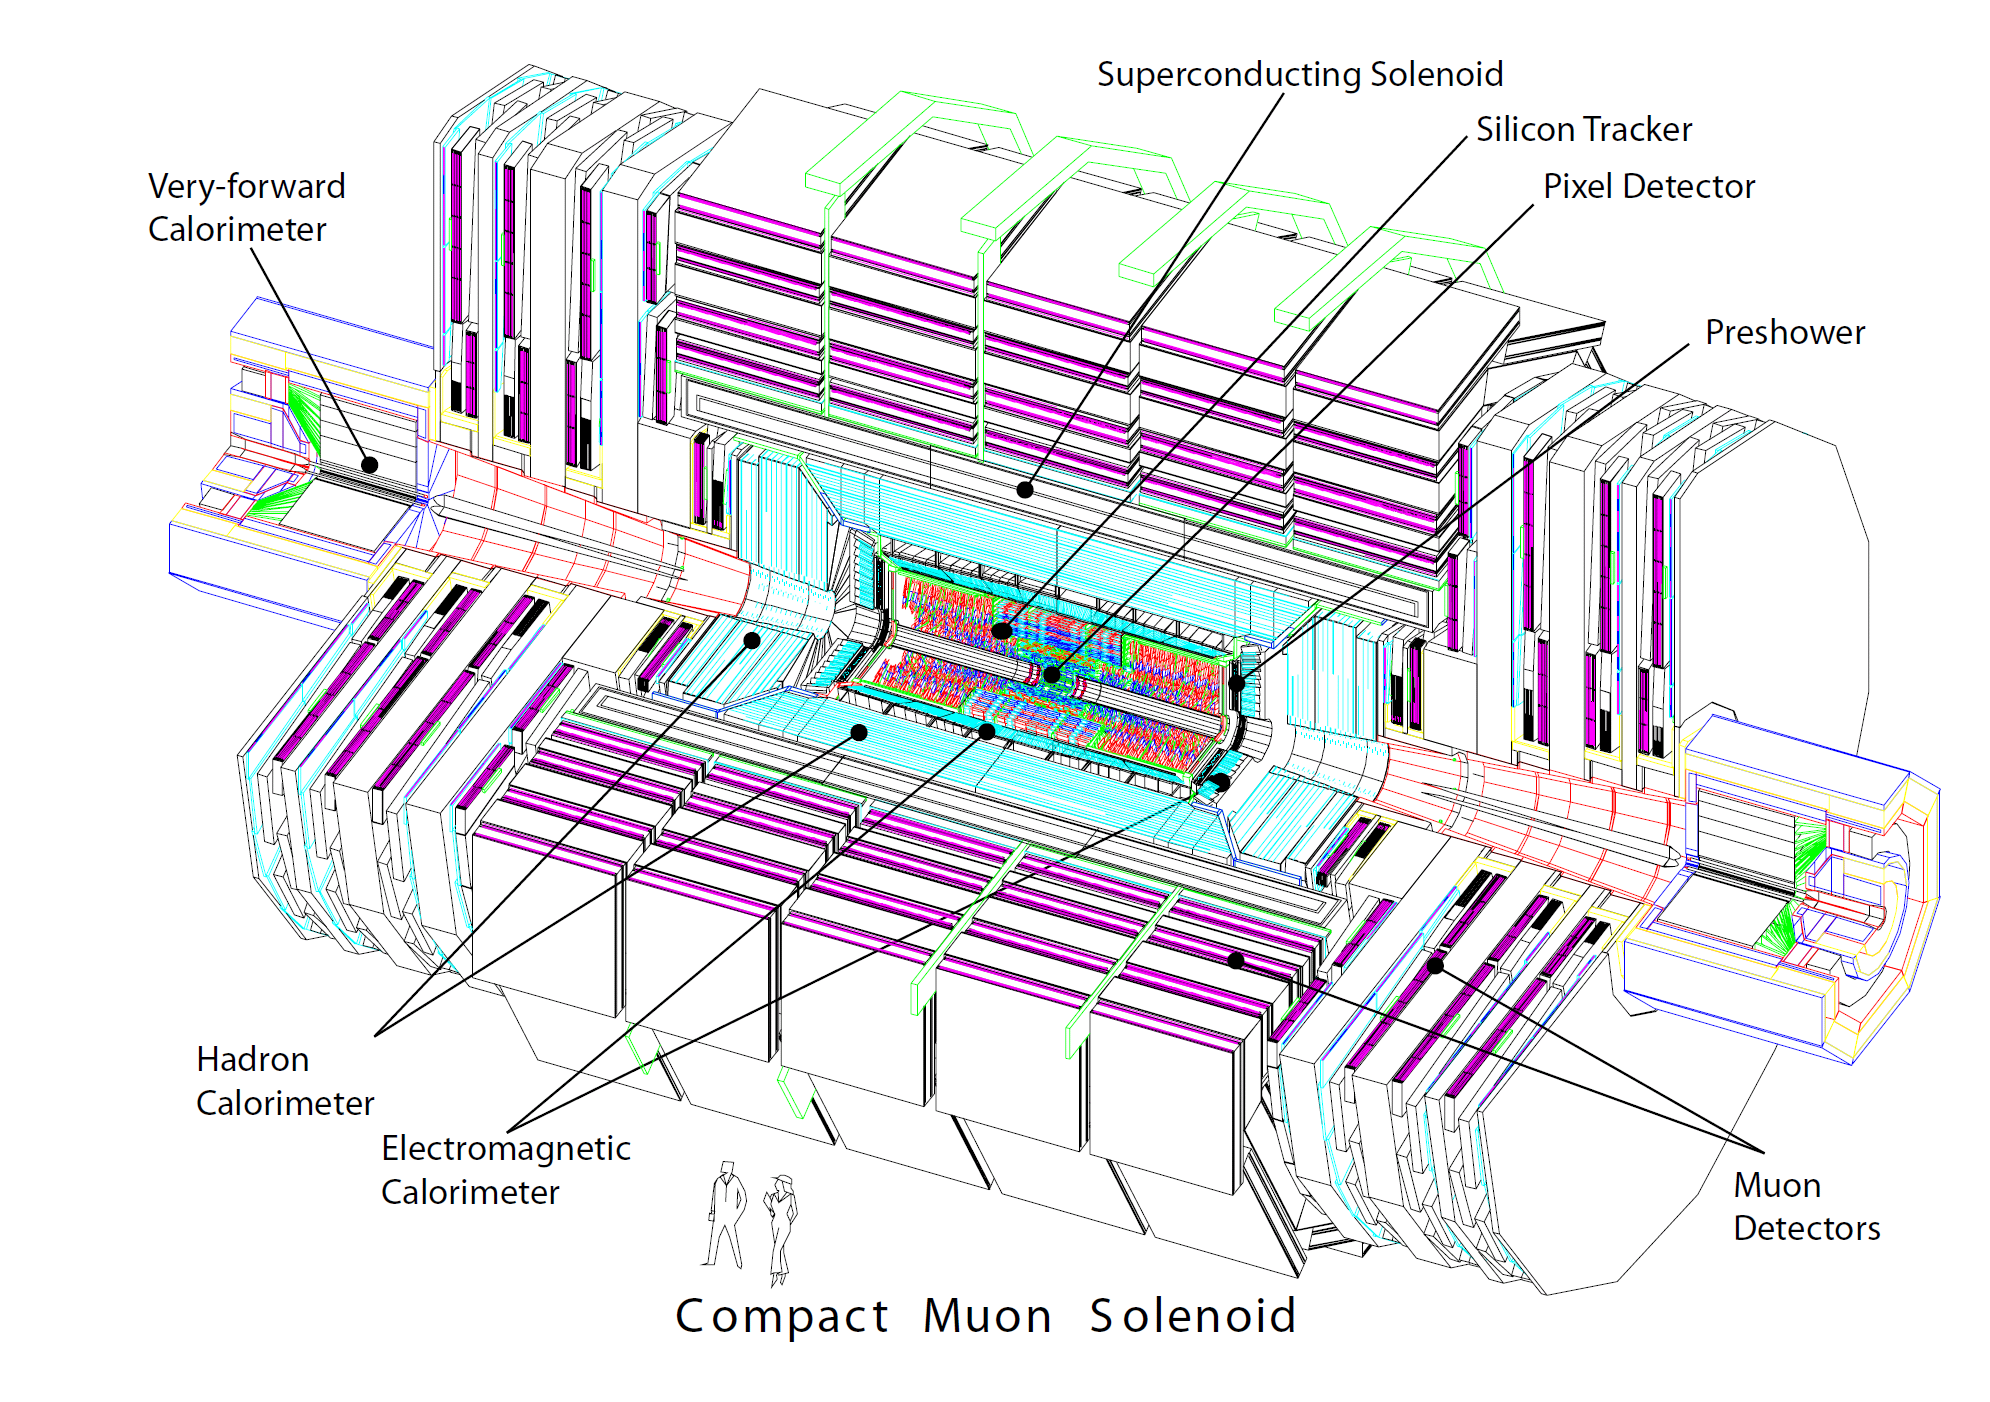
\includegraphics[width=0.75\textwidth]{detector/pics/CMS_apparatus.png}
	\end{tabular}
	\caption{An exploded view of the CMS detector.}
	\label{fig:CMS_apparatus}
\end{figure}

\begin{figure}[tbh!]
	\centering
	\begin{tabular}{cc}
		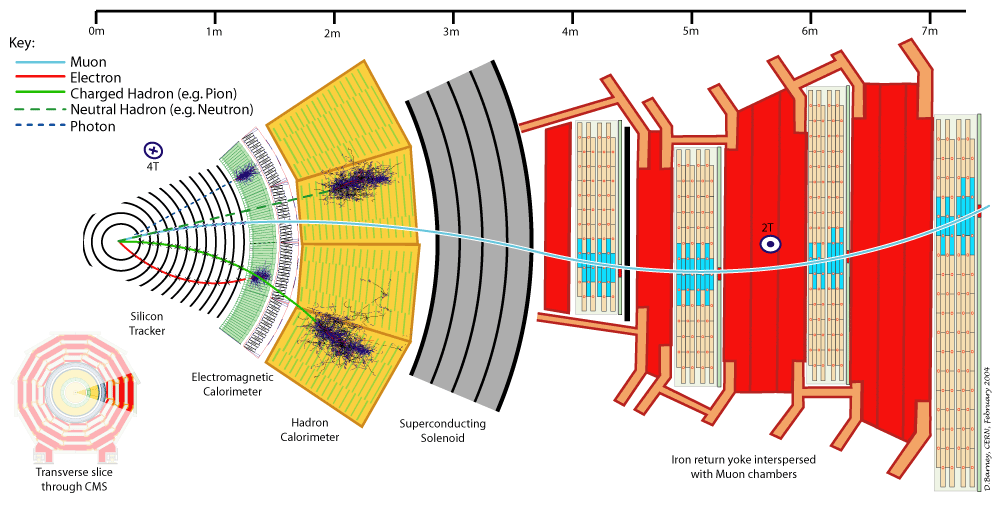
\includegraphics[width=0.75\textwidth]{detector/pics/CMS_slice.png}
	\end{tabular}
	\caption{Longitudinal section of the CMS detector showing the different detectors components and position.}
	\label{fig:CMS_slice}
\end{figure}

\subsection{Inner tracking system}

The Inner Tracking systems reconstructs the track of charged particles and measures their momentum. In order to meet the design requirements of a compact design and high reconstruction efficiency ($95\%$ for high momentum $\mu$ particles) the main detector material is silicon.
The detector can be easily divided in three parts:
\begin{itemize}
	\item Placed close to the interaction point where the particle flux is higher are the pixel detectors. Each pixel is 100×150 $\mu m^{2}$ wide;
	\item In the intermediate region ($20 < r < 55 cm$) the particle flux is low enough to allow the usage of silicon micro-strips, with each cells with the minimum size of $10 cm × 80 \mu m$;
	\item in the outermost region ($r > 55 cm$),the particle flux is low enough to allow bigger size micro-strips with size of $25 cm × 180 \mu m$ 
\end{itemize}

A section of the whole Inner Tracking apparatus on the z-plane is viewable in Figure \ref{fig:Pixel_zview}. Close to the interaction point 3 pixel-layers are placed at radial distances of $4.7$, $7.3$ and $10.2 cm$. In the Barrel region the silicon micro-strips are placed at a radial distance between $20$ and $110 cm$. The forward region has instead 2 pixel and 9 micro-strips layers. The barrel micro-strip section is divided in 2 different parts: the innermost and the outermost one. In order to avoid excessively shallow track crossing angles, the Inner Barrel region is shorter than the Outer one, and there are an additional 3 Inner Disks in the transition region between the Barrel and Endcap parts, on each side of the Inner Barrel. The overall inner layout apparatus is viewable in Figure \ref{fig:Pixel_layout}. The total area of the pixel detector is $\approx 1 m^{2}$, whilst that of the silicon strip detectors is $200 m^{2}$, providing coverage up to $|\eta| < 2.4$. The inner tracker comprises 66 million pixels and $9.6$ million silicon strips. The silicon pixels grants a precision of $10 \mu m$ on the $(x,y)$ transverse plane and of $20 \mu m$ on the z axis. The resolution of the silicon micro-strips depends on each cell thickness, with a minimum value of $ 55 \mu m$ for the traverse plane.


\begin{figure}[tbh!]
	\centering
	\begin{tabular}{cc}
		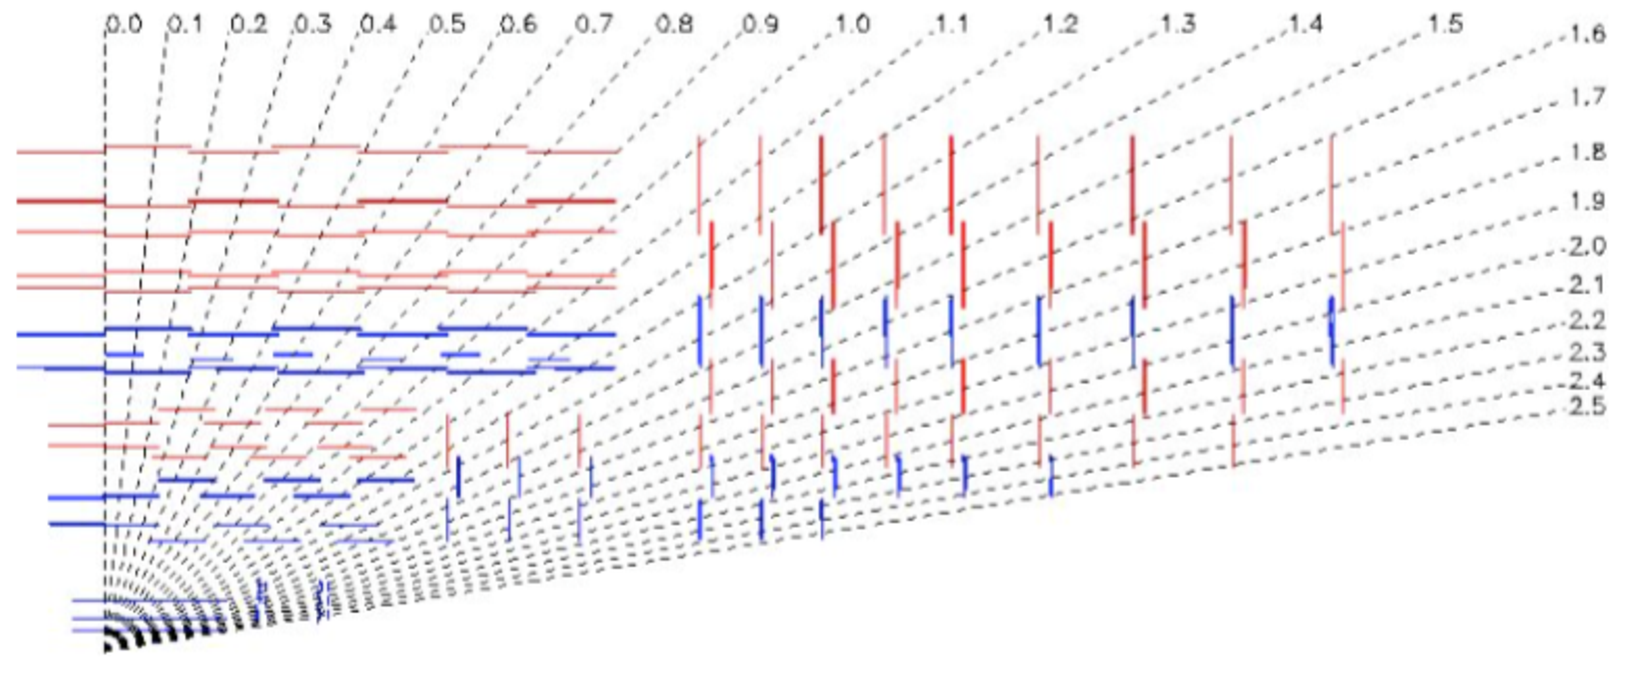
\includegraphics[width=0.75\textwidth]{detector/pics/Pixel_zview.pdf}
	\end{tabular}
	\caption{The tracker layout (1/4 of the z view).}
	\label{fig:Pixel_zview}
\end{figure}

\begin{figure}[tbh!]
	\centering
	\begin{tabular}{cc}
		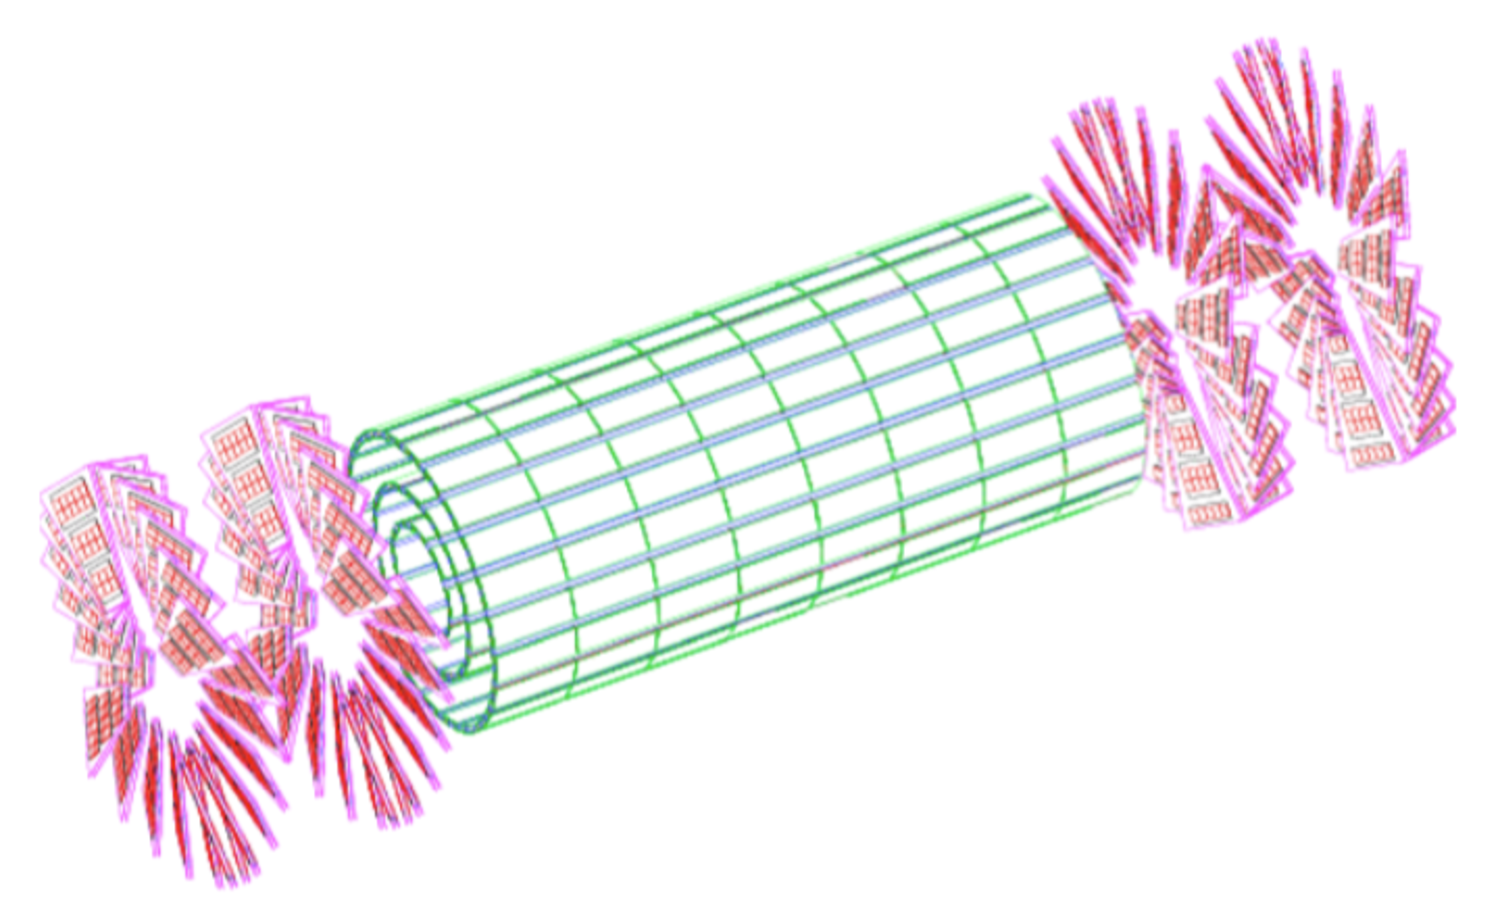
\includegraphics[width=0.75\textwidth]{detector/pics/Pixel_layout.pdf}
	\end{tabular}
	\caption{Layout of pixel detectors in the CMS tracker.}
	\label{fig:Pixel_layout}
\end{figure}

\subsection{The Electromagnetic calorimeter}

The Electromagnetic Calorimeter (ECAL) is a hermetic, homogeneous calorimeter comprising 61200 lead tungstate ($PbWO_{4}$) crystals mounted in the central barrel part, closed by 7324 crystals in each of the 2 endcaps.
The the crystal material choice was driven by the short radiation length and Molière ray, granting compactness and good granularity as listed on Table \ref{table:CMS_PbWO4}. Other $PbWO_{4}$ important properties are radiation resistance and the short decaying time witch allows to collect the $85\%$ of light during the $25$ ns interval between a bunch crossing and the next one.

\begin{figure}[tbh!]
	\begin{center}
		
		\begin{tabular}{ | l | c |}
			\hline
			Density  & $ 8.28 g/cm^{3}$ \\ \hline
			$X_{0}$   & $0.89 cm$  \\ \hline
			$R_{M}$ 2.2 & $2.2 cm$  \\ \hline
			\hline
		\end{tabular}
		\caption{Parameters of the $PbWO_{4}$ crystals .}
		\label{table:CMS_PbWO4}
	\end{center}
\end{figure}

The Ecal is made of a central body in the Barrel region and two identical structures covering the Endcap ones. The final design aim was to build a calorimeter as compact as possible. In order to have high hermeticity the space in between crystals has been reduced as much as possible especially in the transition region between Barrel and Endcaps. 

The Barrel covers a pseudo-rapidity region of $|\eta| < 1.479$ with its cylinder ray of 129 cm. It contains 61200 crystals; 360 placed in $\phi$ and $2\times85$ in $\eta$. The crystals are quasi-projective (the axes are tilted at $3^{\circ}$ with respect to the line from the nominal vertex position) and cover $0.0174$ (i.e. $1^{\circ}$) in $\Delta\phi$ and $\Delta\eta$. The crystals have a front face cross-section of $\approx 22\times22 mm^{2}$ and a length of 230 mm, corresponding to $25.8 X_{0}$. The Endcaps cover the pseudo-rapidity of $1.48 < |\eta| < 2.6$ where the $2.6\times2.6\times22 cm^{3}$ are gathered in $5\times5$ matrices called supercrystals.

In the pseudo-rapidity interval of $1.653 < |\eta| < 2.56$, as shown on Figure \ref{fig:ECAL_section}, is present a detector called Preshower, halo-ring shaped. The preshower is a sampling calorimeter made by two distinct layers; the showering layer made of lead and the detector layer made of silicon strips capable of measuring the energy deposit of the initial part of particle showers as well as their lateral profile. The role of this detector is important whenever multiple particle showers overlap in the ECAL Endcap allowing a clear distinction of each of those showers.

The overall ECAL resolution can be parametrized as a function of the energy measured:

\begin{equation}
\dfrac{\sigma}{E}^{2} = \dfrac{S}{\sqrt{E}}^{2} + \dfrac{N}{E}^{2} + C^{2}
\end{equation}

where S is the stochastic term, N the noise and C the constant term. The values of these
parameters are listed on Figure \ref{fig:ECAL_resolution}.  

\begin{figure}[tbh!]
	\centering
	\begin{tabular}{cc}
		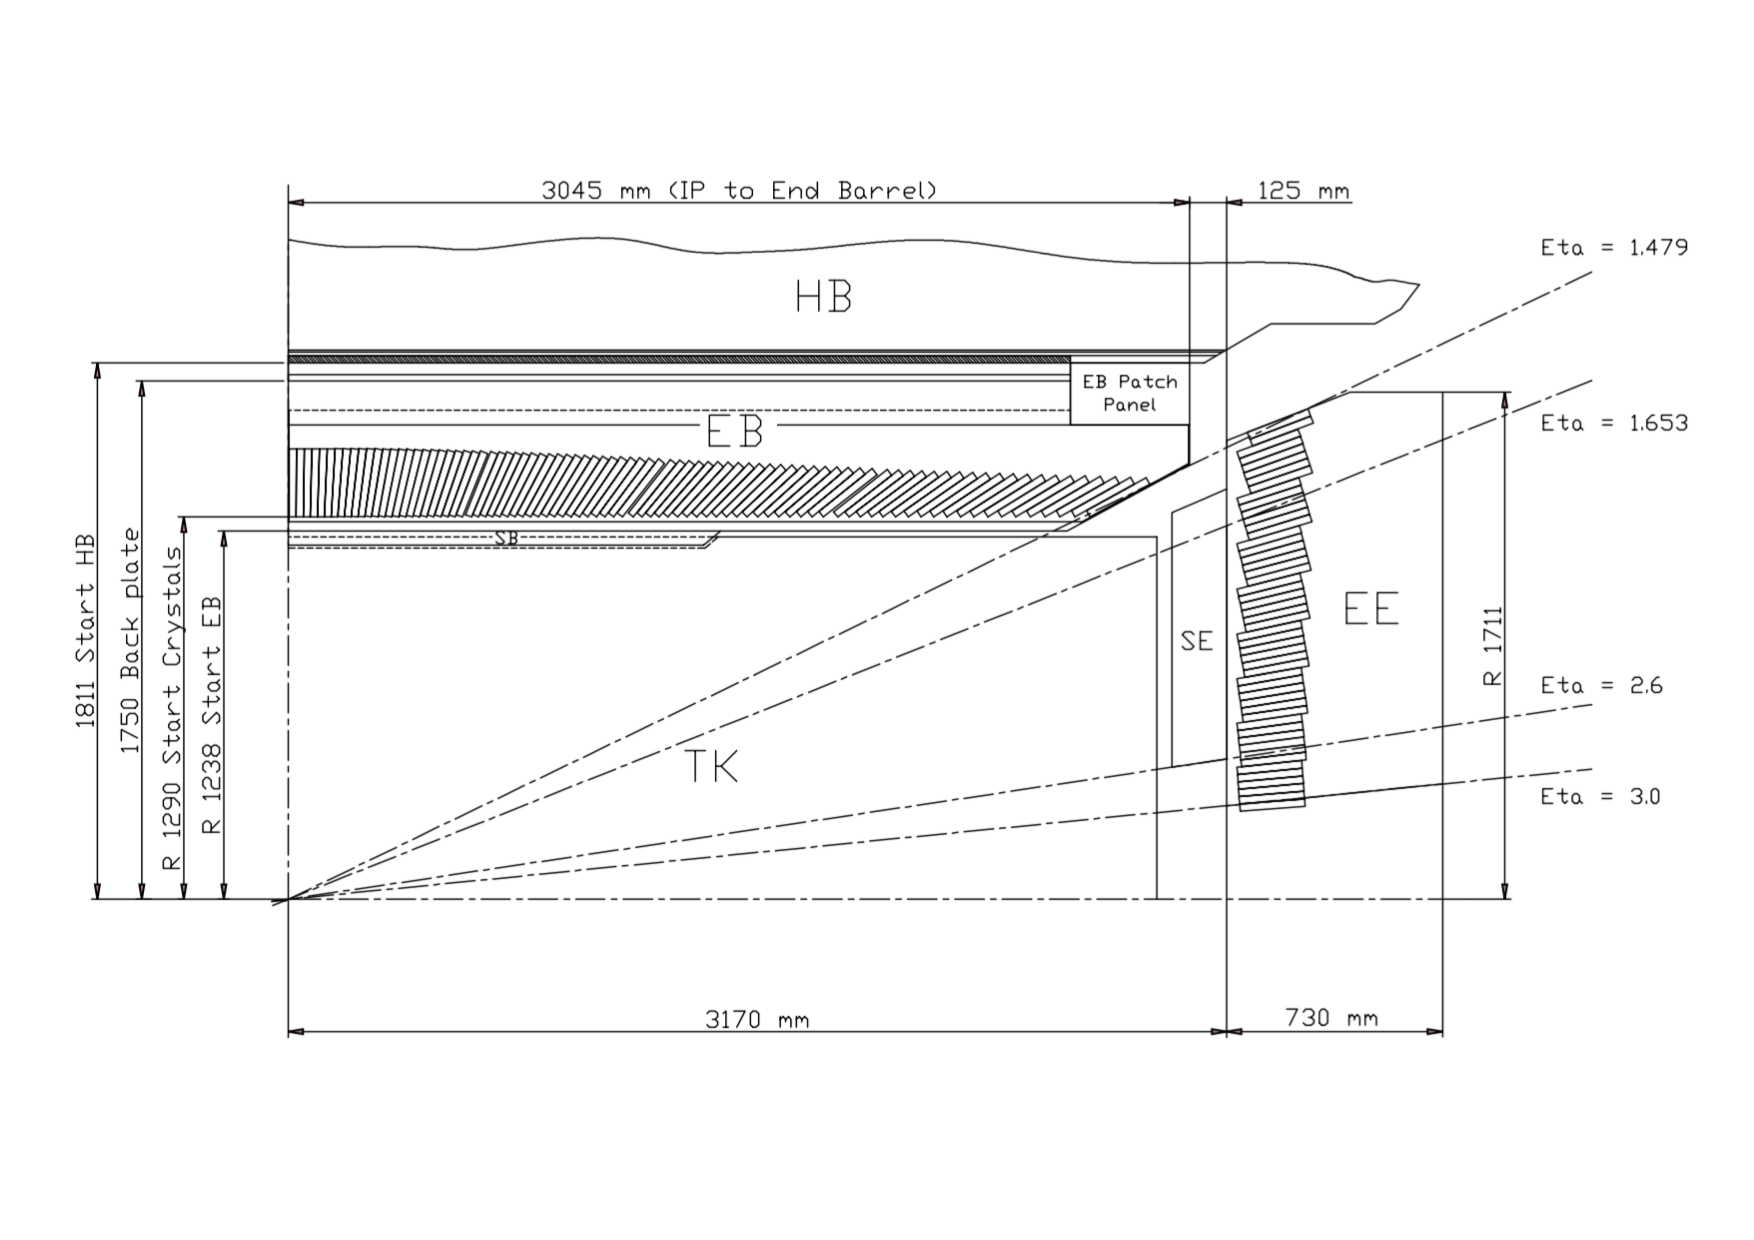
\includegraphics[width=0.75\textwidth]{detector/pics/ECAL_section.pdf}
	\end{tabular}
	\caption{Longitudinal section of the electromagnetic calorimeter (one quadrant).}
	\label{fig:ECAL_section}
\end{figure}

\begin{figure}[tbh!]
	\centering
	\begin{tabular}{cc}
		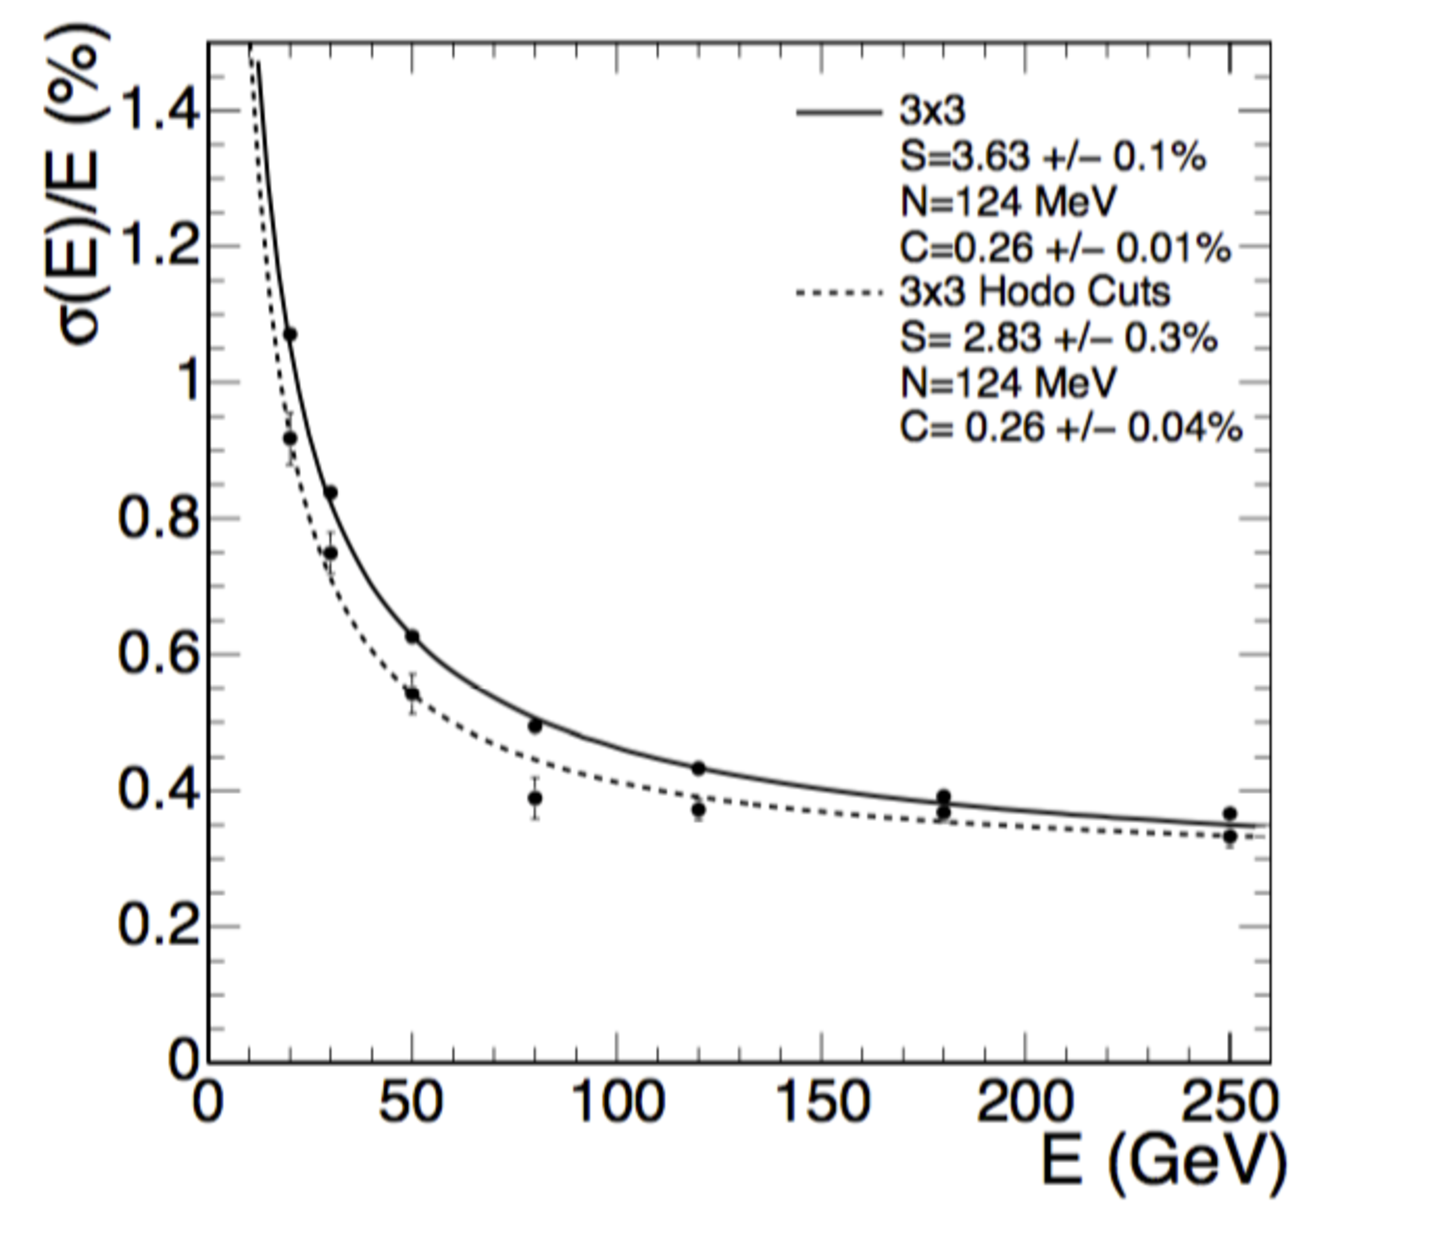
\includegraphics[width=0.75\textwidth]{detector/pics/ECAL_resolution.pdf}
	\end{tabular}
	\caption{ECAL supermodule energy resolution, $\sigma_{E}/E$, as a function of electron energy as measured from a beam test. The upper series of points correspond to events taken with a $20x20 mm^{2}$ trigger and. The lower series of points correspond to events selected to fall within a $4x4 mm^{2}$ region. The energy was measured in an array of $3x3$ crystals with electrons impacting the central crystal.}
	\label{fig:ECAL_resolution}
\end{figure}

\subsection{The Hadron calorimeter}

The Hadronic Calorimeter (HCAL) is used along side with the electromagnetic one in order to measure the energy deposit and position in the detector for hadronic jets, the transverse energy and the missing transverse energy $\met$. The requirements for this detector are to minimize as much as possible the Gaussian tail of the resolution distribution and good containment of the hadronic showers in order to have good $\met$ measurements. Its design is influenced by the choice of the magnet parameters since is located inside the superconducting magnet along with the ECAL and the inner tracking system. 

The hadron Barrel (HB) part of HCAL consists of 32 towers covering the pseudo-rapidity region $−1.4 < \eta < 1.4$, resulting in 2304 towers with a segmentation $\Delta\eta\times\Delta\phi = 0.087\times0.087$, corresponding to a $5x5$ ECAL crystal tower. The HB is constructed in 2 half barrels. The HB is readout as a single longitudinal sampling. There are 15 brass plates, each with a thickness of about 5 cm, plus 2 external stainless steel plates for mechanical strength. Particles leaving the ECAL volume first see a scintillator plate with a thickness of 9 mm rather than 3.7 mm for the other plates. The light collected by the first layer is optimized to be a factor of about 1.5 higher than the other scintillator plates. The radiation length $\lambda_{0}$ for HB is $8.9$.

Each hadron Endcap (HE) of HCAL consists of 14 $\eta$ towers with $5^{\circ}$ $\phi$ segmentation,covering the pseudo-rapidity region $1.3 < |\eta| < 3.0$. For the 5 outermost towers (at smaller $\eta$) the $\phi$ segmentation is $5^{\circ}$ and the $\eta$ segmentation is 0.087. For the 8 innermost towers the $\phi$ segmentation is $10^{\circ}$, whilst the $\eta$ segmentation varies from 0.09 to 0.35 at the highest $\eta$. The total number of HE towers is 2304. The radiation length $\lambda_{0}$ for HE is $10.0$.

In order to improve the shower containment there's another calorimeter, called "Tail catcher" placed right outside the magnet. As further hermeticity improvement a "forward" calorimeter (HF) has been installed at around $11$ meters from the interaction point, covering the $\eta$ region of $3.0 < |\eta| <5.0$. This calorimeter is made of steel/quartz fibres running paralel to the beam line.

Figure \ref{fig:HCAL_section} shows the longitudinal section of the HCAL and the locations of its parts HB, HE, HF and HO.

The HCAL energy resolution is:

\begin{equation}
\dfrac{\sigma(E)}{E} = \dfrac{100\%}{\sqrt{E}}\oplus 4.5\%
\end{equation}

\begin{figure}[tbh!]
	\centering
	\begin{tabular}{cc}
		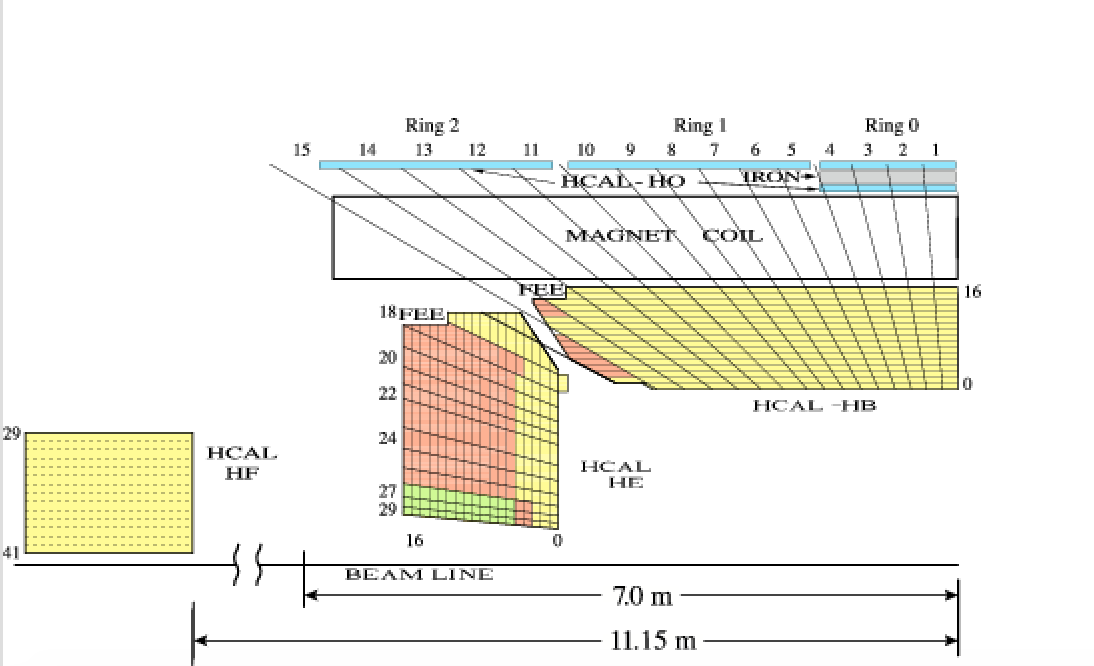
\includegraphics[width=0.75\textwidth]{detector/pics/HCAL_section.png}
	\end{tabular}
	\caption{The CMS HCAL detector (quarter slice). "FEE" indicates the locations of the Front End Electronics for HB and HE. The signals of the tower segments with the same color are added optically, to provide the HCAL "longitudinal" segmentation. HB, HE and HF are built of 36 identical azimuthal wedges\,($\Delta\phi = 20$ degrees).}
	\label{fig:HCAL_section}
\end{figure}

Table \ref{fig:HCAL_resolution} shows the distribution of the jet energy resolution as function of the simulate jet traverse energy.

\begin{figure}[tbh!]
	\centering
	\begin{tabular}{cc}
		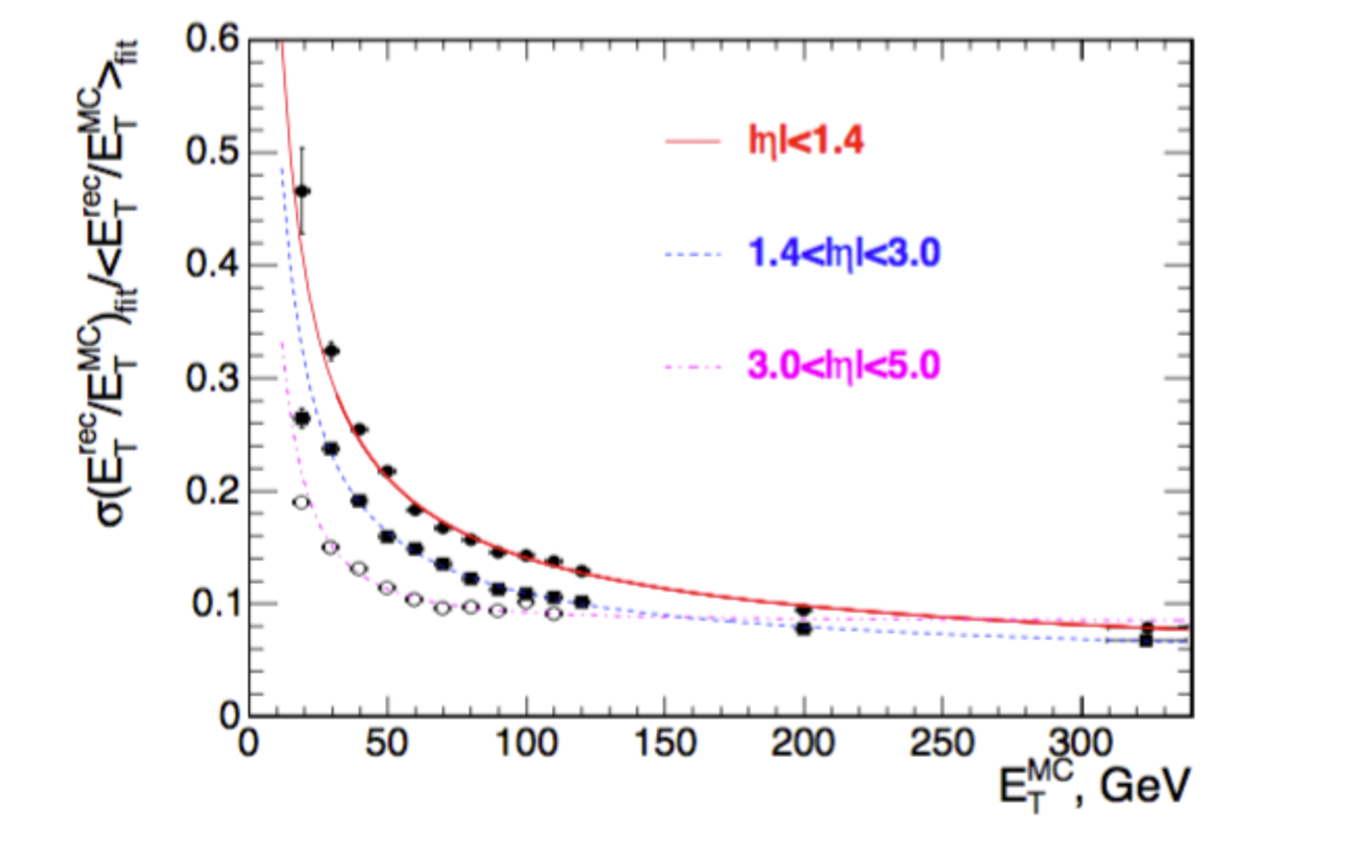
\includegraphics[width=0.75\textwidth]{detector/pics/HCAL_resolution.pdf}
	\end{tabular}
	\caption{The jet transverse energy resolution as a function of the simulated jet transverse energy for barrel jets $(|\eta| < 1.4)$, endcap jets $(1.4 < |\eta| < 3.0)$ and very forward jets $(3.0 < | \eta | < 5.0)$. The jets are reconstructed with the interative cone $R = 0.5$ algorithm.}
	\label{fig:HCAL_resolution}
\end{figure}

\subsection{The Magnet}

The precision requirements of the muon chambers in order to distinguish unambiguously $\approx 1$ TeV/c muon charge is $\Delta p / p \approx 10\%$ therefore the requirement of a magnetic field with high bending power.
The CMS magnet is large superconducting solenoid, the parameters of which are given in Table \ref{table:CMS_magnet}. A large bending power can be obtained for a modestly-sized solenoid as the bending starts at the primary vertex. A good length/radius ratio is necessary to ensure good momentum resolution in the forward region as well.

\begin{figure}[tbh!]
	\begin{center}
	
		\begin{tabular}{ | l | l |}
			\hline
			Field & 4 T \\ \hline
			Inner Bore & 5.9 m \\ \hline
			Length & 12.9 m \\ \hline
			Number of Turns & 2168  \\ \hline
			Current & 19.5kA   \\ \hline
			Stored Energy & 2.7 GJ  \\ \hline
			Hoop Stress & 64 atm \\
			\hline
		\end{tabular}
		\caption{Parameters of the CMS superconducting solenoid.}
		\label{table:CMS_magnet}
			\end{center}
	\end{figure}

The main features of the CMS solenoid are the use of a high-purity aluminium-stabilised conductor and indirect cooling (by thermosyphon), together with full epoxy impregnation.


\subsection{The Muon System}

Three types of gaseous detectors are used to identify and measure muons \ref{muondetectors}. The choice of the detector technologies has been driven by teo reasons: the high radiation environment and the large surface to cover. Since in the barrel region of $|\eta| < 1.2$, both the muon rate and the residual magnetic field in the chambers is low, drift tube (DT) chambers are used. In the 2 endcaps insted, where the muon rate as well as the neutron induced background rate is high, and the magnetic field is also high, cathode strip chambers (CSC) are placed covering the pseudo-rapidity region up to $|\eta| < 2.4$. Additionally, resistive plate chambers (RPC) are used in both the barrel and the endcap regions covering a pseudo-rapidity region of $|\eta| < 2.1$. These RPCs operate in avalanche mode to ensure good performances at high rates and have double gaps with a gas gap of 2 mm. RPCs provide a fast response with good time resolution but with a coarser position resolution than the DTs or CSCs. RPCs can therefore identify unambiguously the correct bunch crossing.

The DTs or CSCs and the RPCs operate within the first level trigger system, providing independent and complementary sources of information.
The layout of one quarter of the CMS muon system for initial low luminosity running is shown in Figure \ref{fig:CMS_muonsys}. In total, the muon system contains of order 25000 $m^{2}$ of active detection planes, and nearly 1 million electronic channels.

\begin{figure}[tbh!]
	\centering
	\begin{tabular}{cc}
		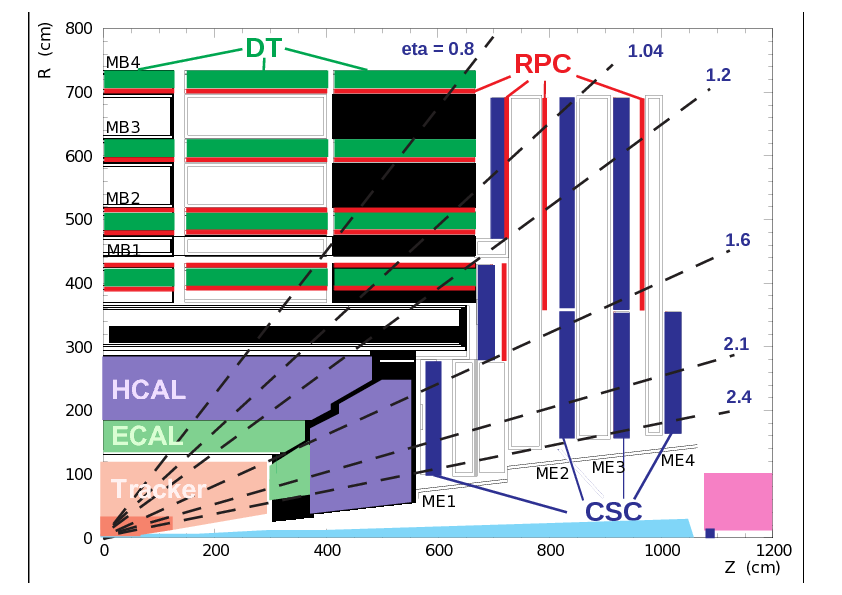
\includegraphics[width=0.75\textwidth]{detector/pics/CMS_muonsys.png}
	\end{tabular}
	\caption{Layout of one quarter of the CMS muon system for initial low luminosity running.
		The RPC system is limited to $|\eta| < 1.6$ in the endcap, and for the CSC system only the inner
		ring of the ME4 chambers have been deployed.}
	\label{fig:CMS_muonsys}
\end{figure}

\subsection{The Trigger System}

With a bunch crossing rate of 40 Mhz at design luminosity and the possibility to record the information for $\approx 10^{2}$ crossings/sec the CMS experiment needs a trigger system capable of a rejeftion factor of at least $10^{6}$.

The CMS trigger and data acquisition system (DAQ) consist of 4 parts: the detector electronics, the hardware-based level 1 trigger, the readout network and and the online event filter system that uses a software-based high level trigger (HLT).

There's a minimum transit time required for the signal to reach the level one trigger hardware based on the service tunnels next to the CMS experiment site, wait for the trigger response to keep or discard the event and send it back to the detectors readout apparatus. The average time needed for a single cycle is 3.2 $\mu s$. During the following time the event information is stored in a buffer waiting for the Level-1 trigger response. The trigger decisional time is less than 1 $\mu s$ with a rejection power of around 1 crossing kept every 1000.

The Level-1 decision is based on "trigger primitive" objects such as photons, electrons and muons and jets above thresholds as well as the transverse energy $E_{T}$ and the missing transverse energy $\met$ involving the calorimetry and the muon system and a combination between these detectors. Since the Level-1 trigger is meant to take fast decisions at a high rate (the design value is 100kHz) the trigger objects are reconstructed with reduced resolution and granularity. A safe time margin of a factor of 3 is taken into account in order to cover for possible reconstruction uncertainties as well as beam and detector conditions leading to a rate of 16kHz. The design value of 100 kHz is set by the average time to transfer full detector information through the readout system. A schematic overview of the Level-1 Trigger structure is shown on figure \ref{fig:trigger_lvl1}.

\begin{figure}[tbh!]
	\centering
	\begin{tabular}{cc}
		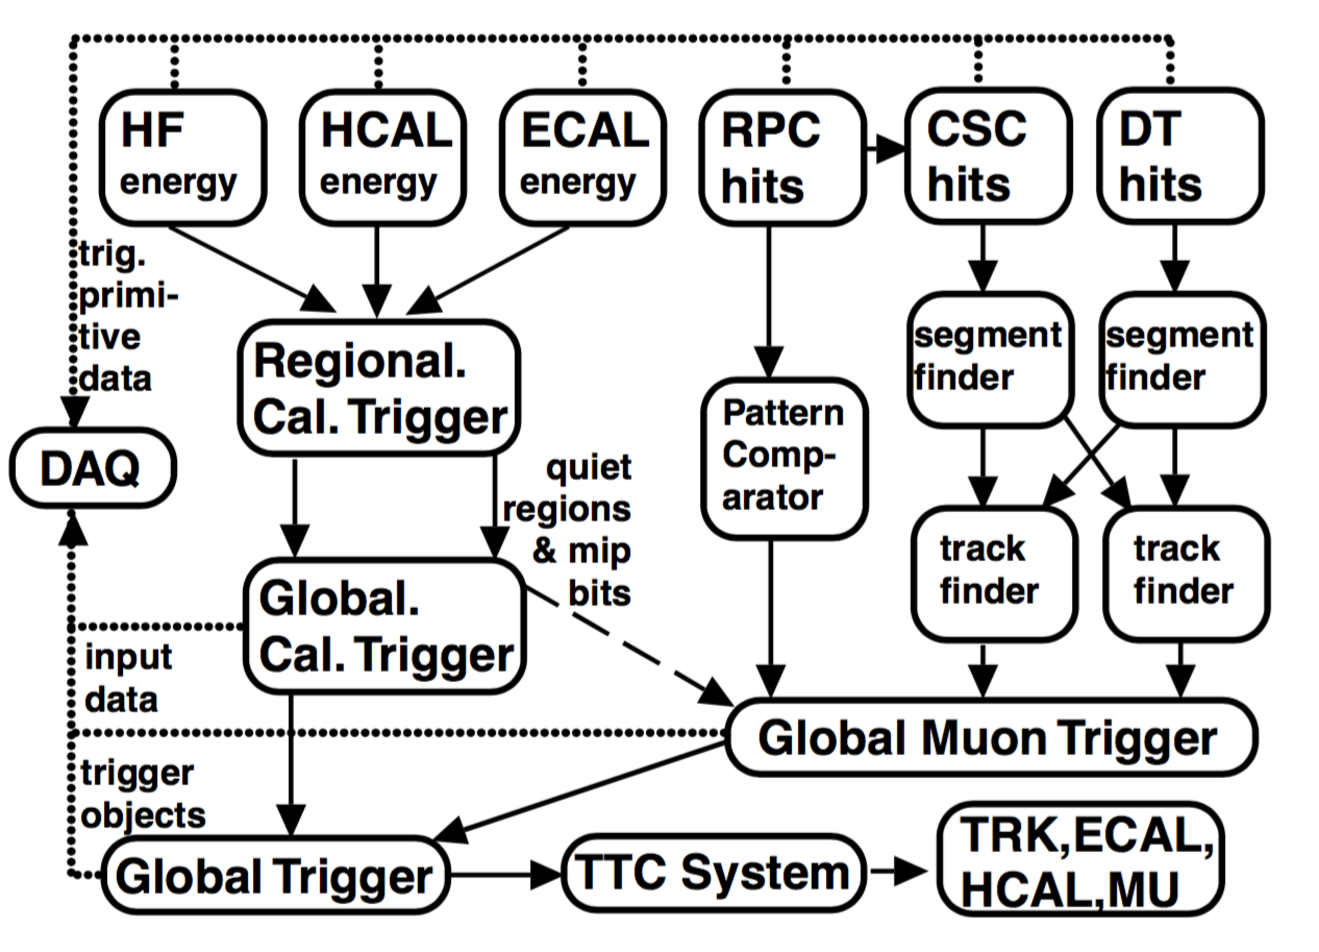
\includegraphics[width=0.75\textwidth]{detector/pics/trigger_lvl1.pdf}
	\end{tabular}
	\caption{Overview of Level 1 Trigger.}
	\label{fig:trigger_lvl1}
\end{figure}

Once an event passes the Level-1 trigger selection the data from the pipelines to the front end readout buffers waiting for a further event reconstruction. After a successful reconstruction the compressed event is sent to one processors of the available farm that runs the same High Level Trigger (HLT) software. The main aim of the HLT is to gather all the informations collected in the event in order to trigger over more complex objects such as $\tau$ particles, multiple jets and multiple particle object or event reconstructed quantities in order to further reduce the event rate from 100kHz to 100Hz for mass storage.

\subsection{Software and Computing}

The CMS software and computing systems covers a broad range of tasks:

\begin{itemize}
	\item online and offline calibration and status reports for each of the subdetectors;
	\item management, maintenance and access of the data storage;
	\item reconstruction and analysis of data;
	\item support of the distributed computing infrastructure and software framework.
\end{itemize}

The scale of the CMS collaboration in terms of storage capabilities, networking power is orders of magnitude higher that the CERN's infrastructure capabilities. Therefore the CMS computing model is highly distributed, with a primary "Tier-0" centered at CERN with the additional support by "Tier-1" and "Tier-2" computing centers scattered worldwide in several universities and research centers. All those facilities as shown on Figure \ref{fig:CMS_grid} have hierarchical structure under the Tier-0 and go under the name of "CMS Computing Grid".

\begin{figure}[tbh!]
	\centering
	\begin{tabular}{cc}
		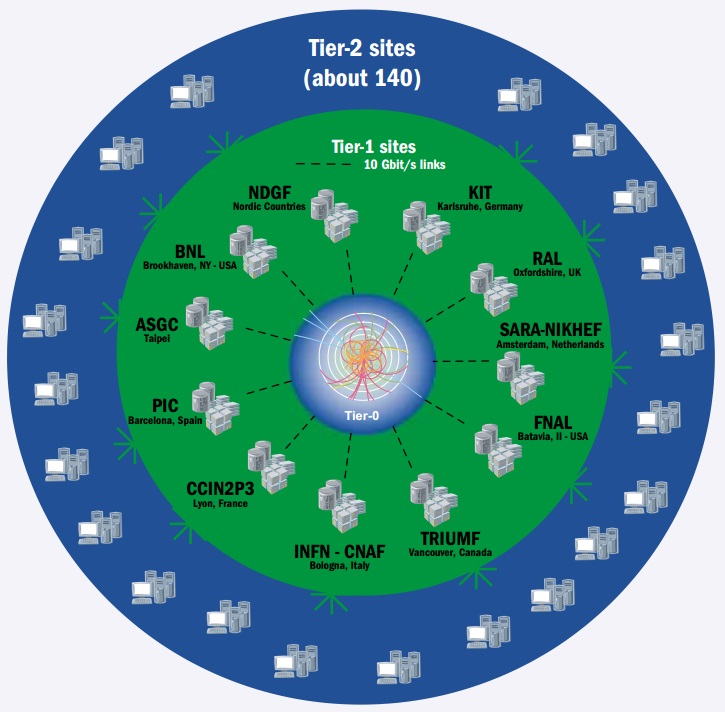
\includegraphics[width=0.75\textwidth]{detector/pics/CMS_grid.jpg}
	\end{tabular}
	\caption{Overview of the structure of the CMS Computing Grid.}
	\label{fig:CMS_grid}
\end{figure}

\section{CMS Detector Upgrades for 13 TeV Run}

We should discuss if it is worth

Figures and Tables list

\begin{itemize}
	\item Summary of the detector upgrades
	\item Pile up regime for 13 TeV
\end{itemize}